% Chapter Template

\chapter{Apport de la structure d’index M-Tree dans un CBIR} % Main chapter title

\label{ChapterX} % Change X to a consecutive number; for referencing this chapter elsewhere, use \ref{ChapterX}

%----------------------------------------------------------------------------------------
%	SECTION 1
%----------------------------------------------------------------------------------------

\section{Introduction}
Dans les systèmes de recherche d'images par le contenu le temps d'exécution d'une requête est d'une importance primordiale. Pour répondre aux besoins d'un CBIR d'être robuste en temps du calcul lors de l'étape d'indexation et l'étapes de recherche de nombreuse méthodes d'indexation ont vu le jour. Parmi ces méthode ou structures on trouve la structure M-tree, une structure recherche par similarité dans les espaces métriques, que nous avons choisi pour la partie d'accélération de recherche dans notre sujet. \\
 
La discussion du sujet de recherche par similarité dans les espaces métriques soulève plusieurs questions. Tout d’abord, les premières questions qui se posent sont des questions sur les espaces métriques comme : quelles sont les propriétés et les caractéristiques des espaces
métriques ? Ensuite, quelles sont les fonctions de similarité qui répondent aux critères des distances métriques? Quels sont les types des requêtes souvent utilisées pour chercher dans les espaces métriques?\\

Enfin, la discussion de recherche par similarité dans les espaces métriques conduit forcément à poser des questions sur les méthodes métriques d’indexation et de recherche, quelles sont les méthodes principales de recherche par similarité dans les espaces métriques
qui sont proposées dans la littérature, et quels sont les avantages et les inconvénients de chaque méthode?

Ce chapitre vise à discuter ce sujet afin de surligner les déférents concepts y liés.
\section{L’espace métrique}
Etant donné un ensemble E des objets, chaque fonction $d: E\times E\rightarrow R^+$ qui satisfait les trois propriétés suivantes est appelée une distance:

\begin{equation}
	\begin{array}{cc}
	(p1) \textbf{La positivité} : & \forall (x,y)\in E^2, d(x,y) \ge 0 \\
	(p2) \textbf{La symétrie} : & \forall (x,y)\in E^2, d(x,y) = d(y,x) \\
	(p3) \textbf{Réflexivité} : & \forall (x,y)\in E^2, d(x,y) = 0 \Rightarrow x = y
	\end{array}
\end{equation}

Une distance métrique est une distance qui satisfait les trois propriétés ci-dessus plus une quatrième propriété. Cette propriété est connue sous le nom « l’inégalité triangulaire », elle est définie formellement comme le suivant :

\begin{equation}
\begin{array}{cc}
(p4)\textbf{ L’inégalité triangulaire :}  & \forall x,y,z\in E, d(x,y)+d(y,z) \geq d(x,z)
\end{array}
\end{equation}

\begin{description}
	\item[Définition 1:] Un espace Métrique $ (E,d) $ est un ensemble $ E $ muni d’une distance métrique $ d $.
\end{description}

Dans le paradigme de recherche par similarité, la distance entre les objets représente le degré de ressemblance entre ses objets, c.à.d si la distance entre deux objets est petite, cela signifie que ces deux objets sont fortement similaires, et par contre, si la distance est assez grande, les objets sont assez dissimilaires.

\subsection{Les requêtes de recherche par similarité dans les espaces métriques}
La recherche d’informations dans une base de données peut se faire par plusieurs manières. Dans la suite de cette partie nous présentons deux types intéressants de requêtes largement utilisées dans la recherche par similarité dans les espaces métriques, il s’agit de la requête intervalle et la requête des k plus proches voisins.

\subsubsection{La requête intervalle (Range Query R(q,r))}
Ce type consiste à sélectionner dans la base tous les objets dont la distance par rapport à l’objet de la requête $ q $ est inférieure au rayon de recherche $ r $. Formellement, on peut définir la requête intervalle de la manière suivante.\\

\textbf{Définition 2:} Soit $ (E,d ) $ un espace métrique, $ q $ un objet requête et $ r $ est un réel  positif. La requête par intervalle $ R(q,r) $ retourne l’ensemble défini par :
\begin{equation}
	R = \left\{ o\in E / d(o, q) \leq r \right\}
\end{equation}

\begin{figure}[H]
	\centering
	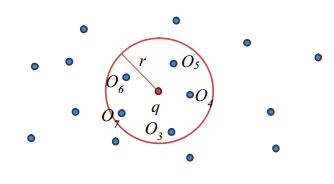
\includegraphics[width=0.65\textwidth]{Figures/rangeQ} % Include the image .png
	\caption{Exemple de la requête intervalle.}
\end{figure}
La Figure 3.1 représente un exemple d’une requête par intervalle dans un espace de
deux dimensions, l’exécution de la requête $ R(q,r) $ retourne le sous-ensemble qui contient les objets $ {O_3,O_4,O_5,O_6,O_7} $.

\subsubsection{La requête des k plus proches voisins kpp (k-NN R(q,k))}
Cette requête consiste à retourner les $ k $ objets les plus similaires à l’objet de la requête $ q $. Formellement, la recherche des $ k $ plus proches voisins est définie comme suite :

\textbf{Définition 3:} Soit $ (E,d ) $ un espace métrique, $ q $ un objet requête, et $ k \in \mathbb{N} $. Alors, la requête  $ R(q,k) $ des $ k $ plus proches voisins $ k $-ppv retourne un sous-ensemble R des objets telle que

\begin{equation}
R = \left\{ o_1,...,o_k \in E / \forall o \in E, d(o, q) \ge \max_{1\leq i \leq k}\left\{d(o_i, q)\right\}  \right\}
\end{equation}

\begin{figure}[H]
	\centering
	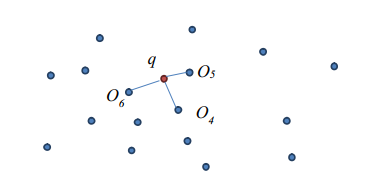
\includegraphics[width=0.65\textwidth]{Figures/knnQ} % Include the image .png
	\caption{Exemple de la requête des k plus proches voisins.}
\end{figure}
La Figure 3.2 représente un exemple d’une requête des k plus proches voisins, l’exécution d’une requête de trois plus proches voisins de la requête q retourne les trois objets $ O_4 $, $ O_5 $ et $ O_6 $.

\subsection{Les fonctions métriques}
Les fonctions métriques sont des fonctions qui permettent de mesurer la distance entre les objets d’un espace métrique. Le choix de la distance métrique convenable de comparaison se fait selon le type des données traitées, en effet, chaque type d’espace métrique à des distances métriques appropriées qui sont spécifiées par les experts. Généralement, les distances métriques sont classifiées en deux catégories [Chávez01]: les distances discrètes et les distances continues. Le choix de distance influence directement sur l’efficacité de la structure utilisée, et le choix de type de distance adéquate, pour construire une telle structure, dépend fortement de la base traitée [Hanif18]. Dans ce qui suit, un aperçu général sur quelques exemples de fonctions métriques continues et des fonctions métriques discrètes.

\subsubsection{Distances Continues}
Les distances continues sont des fonctions métriques qui peuvent retourner un ensemble infini des valeurs. Généralement, elles sont calculées en se basant sur les coefficients des objets. Dans ce qui suit  on donne l'exemples le plus connue des distances continues, La famille des distances de Minkowski Lp est un ensemble des distances continues, elles sont définies formellement par:
\begin{equation}
L_p(I_1, I_2) = \sqrt[p]{\sum_{i=1}^{N}  \left|{I}_{1}(i)-{I}_{2}(i)\right|^p} 
\end{equation}

\begin{itemize}
	\item Manhatttan :  $  L_1(I_1, I_2) = \sum_{i=1}^{N} \left|{I}_{1}(i)-{I}_{2}(i)\right|  $ 
	
	\item Euclidienne : $ L_2(I_1, I_2) =  \sqrt{\sum_{i=1}^{N} \left|{I}_{1}(i)-{I}_{2}(i)\right|^2} $
	
	\item Chebychev : 
	$L_{\infty}(I_1, I_2)=\max_{i=1}^N \left|{I}_{1}(i)-{I}_{2}(i)\right|$  
\end{itemize}

\begin{figure}[H]
	\centering
	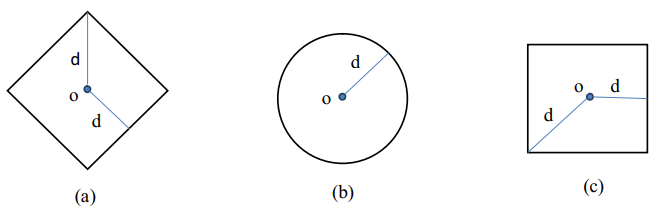
\includegraphics[width=0.5\textwidth]{Figures/mink} % Include the image .png
	\caption{Exemples des distances de la famille Lp:\\ (a) $ L_1 $ (b) $ L_2 $ (c) 	$L_{\infty}$}
\end{figure}

\subsubsection{Distances Discrètes}
Les distances discrètes sont des distances métriques qui ne retournent qu’un nombre limité des valeurs. Généralement, elles sont calculées en se basant sur la comparaison des coefficients des objets pour retourner le nombre des objets qui sont identiques ou le nombre des coefficients qui se diffèrent. Dans la suite de cette section, on présente deux exemples des distances discrètes.

\paragraph{La distance Edit:}
La fonction edit [Levenstein65] est une métrique pour mesurer la distance entre les chaines de caractère. Elle représente le nombre minimal des opérations suffisantes pour convertir une chaine en une autre. Par exemple, on considère deux chaines de caractère $x=x_1x_2...x_n$ et $y=y_1y_2...y_m$, la distance $edit(x,y)$ entre l’objet $x$ et $y$ c’est le nombre des opérations pour convertir la chaine $x$ à $y$. Les opérations qui peuvent être utilisées sur une chaine de caractère sont définies comme suit :
\begin{itemize}
	\item Insérer : pour insérer un caractère dans une position donnée de la chaine
	\item Supprimer : pour supprimer un caractère de la chaine
	\item Remplacer : pour remplacer un caractère d’une position donnée dans la chaine par un autre caractère
\end{itemize}
Edit distance est une distance discrète souvent utilisée pour mesurer la similarité des documents texte et pour manipuler des données scientifiques comme les ADN et les protéines.

\paragraph{La distance de Hamming:}
La distance de Hamming est une distance discrète proposée en 1950 [Hamming50], elle sert à calculer la distance entre les vecteurs. La distance Hamming entre les vecteurs A et B représente le nombre des coefficients qui se diffèrent, si la distance est égale à 0, ça signifie que les vecteurs A et B sont identiques. Formellement, on peut définir la distance de Hamming comme suite:

\begin{equation}
d_h((x_1,...,x_n), (y_1,...,y_n)) = card(\left\{ i: x_i \neq y_i, 1\leq i \leq n\right\})
\end{equation}
Par exemple, la distance de Hamming entre les deux vecteurs $ (1,2,1,3) $ et $ (0,2,3,1) $, et la distance de Hamming entre les deux chaines de caractères « BFEC » et « BFAC » sont calculées comme suit :

\begin{tabular}{cc}
	 $ d_h ((1,2,1,3), (0,2,3,1))= Card({1,3,4}) = 3 $ &  $d_h(BFEC , BFAC)= Card({3}) = 1 $ \\
	 \\
\end{tabular}

L’utilisation de la distance de Hamming est très large [Deza09], elle peut être utilisée pour mesurer de similarité de déférent type des donnés comme images, DNA, Protéine et Textes.

\section{Les données métriques}
La plupart des données acquises aujourd’hui peuvent être modélisées  des objets dans un espace métrique muni d’une distance métrique. Dans cette section, nous présentons des exemples des types bases de données qui peuvent utiliser des distances métriques pour faire la recherche par similarité.

\subsection{Les images 2D}
L’extraction automatique des caractéristiques d'images directement à partir de leur contenu numérique est une solution parmi les solutions possibles pour gérer efficacement les bases de données d'images. Chaque image est représentée par un ou plusieurs vecteurs qui représentent leurs contenus visuels. Par conséquence, la similarité entre deux images peut être mesurée par la comparaison entre leurs descripteurs. La génération d’une base de descripteurs des images représente une phase nécessaire dans les systèmes de recherche d’image par contenu. La description de contenu d’image est souvent faite par des descripteurs de bas niveau, appelés aussi vecteurs caractéristiques, tels que la couleur, la texture et la forme.

\begin{figure}[H]
	\centering
	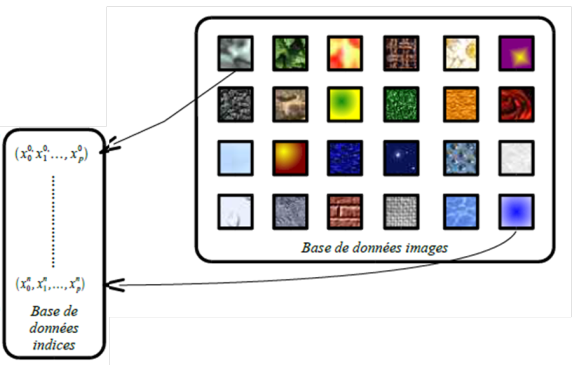
\includegraphics[width=0.55\textwidth]{Figures/horsligne.png} % Include the image .png
	\caption{Exemple de la représentation vectorielle d'une base d'image et d'une image requête.}
\end{figure}
La Figure 3.4 représente un exemple de l’extraction du contenu visuel des images sous forme des vecteurs ; A partir d’une base d’image on peut obtenir une base des vecteurs caractéristiques (indexes) qu’on peut comparer par des distances métriques.

Les distances de Monkowski sont beaucoup utilisées pour mesurer la similarité entre les descripteurs, notamment la distance Euclidienne. 

%\subsection{Séquences d’ADN}
%L'ADN contient les instructions pour toutes les fonctions d’une cellule d’un organisme, deux séquences d’ADN similaires de deux cellules signifient que les deux cellules ont des fonctions similaires. La compréhension de la relation entre une requête d’ADN avec des séquences génomiques, déjà traitées, analysées et stockées dans une base de données, sert à aider les biologistes de bien estimer les fonctionnements de la séquence requête avant de la traiter. La structure d’ADN consiste d’une chaine linéaire des quatre nucléotides qui sont souvent représentés par quatre Alphabets A, C, G et T. La Figure II-6 montre un exemple d’une
%représentation d’un gène humain [WilliamsZobel02].
%
%\begin{figure}[H]
%	\centering
%	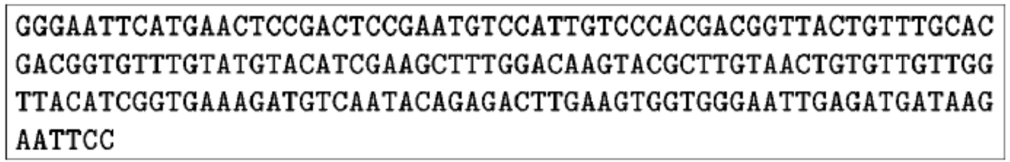
\includegraphics[width=0.55\textwidth]{Figures/ADN} % Include the image .png
%	\caption{Une partie de gène de croissance épidermique humain.}
%\end{figure}
%
%Les séquences génomiques peuvent se modéliser comme un espace métrique muni d’une distance métrique comme la distance Edit et la distance de Hamming.

\section{Les méthodes d’accès Métriques}
L'objectif principal des méthodes d’accès métrique (MAM) est la minimisation du temps de recherche. Le calcul de distance entre les objets métriques est souvent coûteux et consomme beaucoup du temps. Par exemple, le calcul des distances de Minkowski consomme un temps de complexité linéaire, le calcul de la distance Edit entre deux chaines de taille m et n est d’ordre $ O(n\times m) $. De même, la complexité de la distance de Hamming est d’ordre $ O(n\times m) $,certaines distances usuelles peuvent atteindre une complexité d’ordre $ O(n^4)  $ comme la distance Edit-tree [Zezula06]. Donc, la complexité de comparaison d’objets dans une base est un critère crucial qui influence directement sur la performance de la structure métrique utilisée. La mesure de performance se calcule en fonction du nombre de distances calculées lors du parcours de structure pour répondre à une requête parce que la complexité des autres parties des algorithmes de recherche est négligeable devant la complexité de calcul de distance [Chávez01].\\

Le but de MAMs vise à minimiser le nombre de distances calculées lors du stockage et lors de la recherche par l’exploitation des distances pré-calculées et en évitant le parcours des régions inutiles sans faire des calculs supplémentaires. La Figure 3.5 illustre un exemple de cette approche dans les bases de données d’images [Chávez01].\\


La technique la plus simple pour éviter le calcul des distances est l’exploitation directe de l’inégalité triangulaire. Supposons que, les distances entre objet pivot $ p $ des objets $ o_i $ sont pré-calculées, la distance entre une requête $ q $ et les objets $ o_i $ peut être estimée sans besoin du calcul direct des distances, il suffit de calculer la distance $ d(q,p) $ entre la requête et le pivot, ensuite, toutes les distances $ d(q,o_i) $ sont majorées par $ d(q,p)+d(p,o_i) $, et avec un simple effort de calcul nous pouvons déduire que la distance $ d(q,o_i) $ est minorée par $ |d(q,p)-d(p,o_i)| $. En effet, si $ q $ présente un objet requête, $ p $ un objet pivot et $ o $ un objet de la base. Si la distance $ d(q,p) $ entre la requête et le pivot est déjà calculée et la distance entre l’objet $ o $ et le pivot est pré-calculée. On peut estimer la distance entre la requête et l’objet par la formule suivante 
\begin{equation}
    d(q,p)+d(p,o) \geq d(q,o) \geq |d(q,p)-d(p,o)|
\end{equation}

\begin{figure}[H]
	\centering
	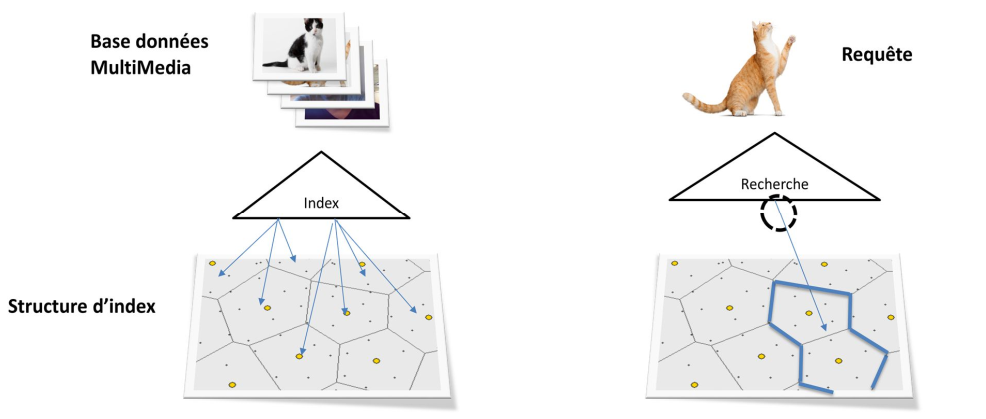
\includegraphics[width=0.6\textwidth]{Figures/similarity.png} % Include the image .png
	\caption{Modèle d'indexation métrique et la recherche par similarité.}
\end{figure}

Lors de la recherche par une requête intervalle $ R(q,r) $, les bornes supérieures et inférieures peuvent être utilisées pour accélérer la recherche. Trois situations sont possibles : si la borne supérieure est inférieure à $  r (d(q,p)+d(p,o) \leq r ) $ alors il est sûr que l’objet $ o $ est pertinent car il vérifie $ d(q,o) \leq r $, si la borne inferieure dépasse le rayon $ r ( |d(q,p)-d(p,o)| > r )  $ alors il est sûr que $ d(q,o) > r $ et par conséquence l’objet $ o $ ne peut être parmi les résultats de la requête. La dernière situation est le pire des cas, il correspond au cas où la borne supérieure est supérieure à $ r $ et la borne inférieure est inférieure à  $ r $  $  (d(q,p)+d(p,o) \geq d(q,o)\geq |d(q,p)-d(p,o)|) $, il est indispensable de calculer la distance $ d(q,o) $ pour déterminer si l’objet $ o_i $ est pertinent ou non.

\begin{figure}[H]
	\centering
	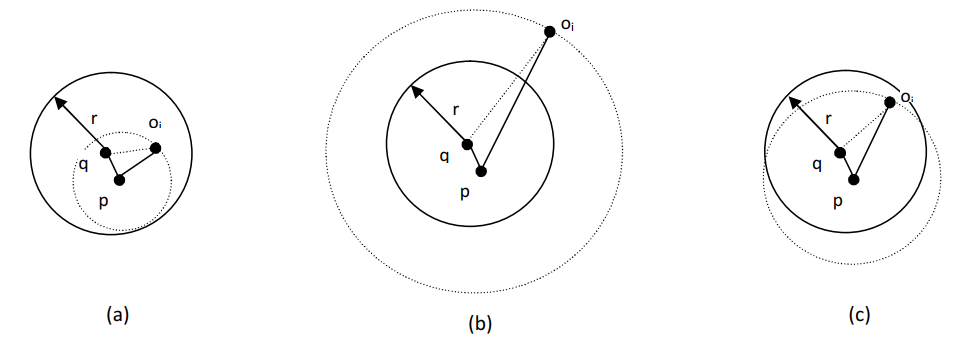
\includegraphics[width=0.6\textwidth]{Figures/pivot.png} % Include the image .png
	\caption{Filtrage par un pivot: (a) l'objet $  o_i $ fait partie du résultat (b) l'objet $ o_i $ sera éliminé (c) le calcul de la
		distance $ d(q,o_i) $ est obligatoire pour savoir si $ o_i $ est pertinent ou pas.}
\end{figure}

Les lignes solides représentent les distances connues, tandis que les lignes coupées représentent les distances non connues.\\

Pour une structure métrique qui utilise un groupe de pivots $ (p_1,p_2,…, p_n) $, les distances entre les objets $ o_i $ et les pivots sont calculées et stockées au préalable. Ainsi, lors d’une recherche par requête intervalle $ R(q,r) $, chaque objet de la base qui satisfait la condition $ \max_{i=1,..,n}{|d(q,pi)-d(o,pi)|} > r $ est certainement non pertinent et donc il sera écarté de la recherche sans aucun calcul de distance. Comme nous avons vu précédemment, le filtrage par n pivots est vu comme un « mapping » de l’espace métrique $ (E,d) $ vers un espace vectoriel $ (R^n, L_\infty) $ en lequel chaque élément $ o \in E $ est représenté par le vecteur $ (d(o,p_1), d(o,p_2),..., d(o,p_n)) $, tout objet $ o $ qui satisfait la condition $ L_\infty((d(o,p_1),..., d(o,p_n)),(d(q,p_1),..., d(q,p_n))) > r  $ sera ignoré durant la résolution d’une requête de rayon $ r $.

\begin{figure}[H]
	\centering
	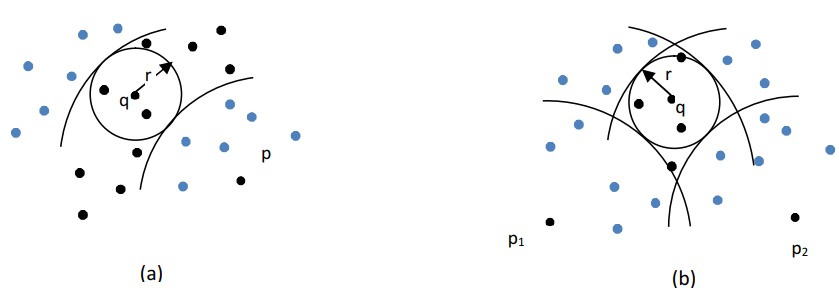
\includegraphics[width=0.6\textwidth]{Figures/npivot.png} % Include the image .png
	\caption{(a) exemple de filtrage par un pivot et (b) par deux pivots.}
\end{figure}

L’utilisation directe des pivots nécessite le stockage des distances entres les pivots et les objets dans la mémoire. Par conséquence, cette technique est coûteuse en termes de la mémoire de stockage. Pour cette raison, d'autres techniques ont été développées pour traiter ce problème comme la technique d’utilisation de double pivot et la technique de regroupement des objets dans des Clusters [Hanif18].


\begin{figure}[H]
	\centering
	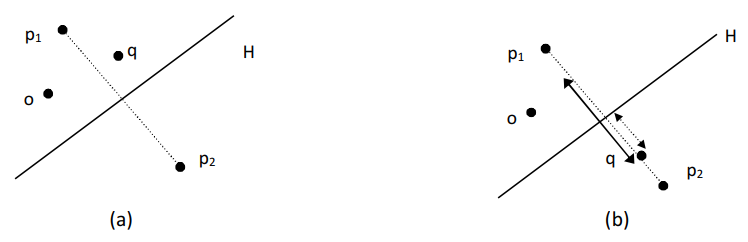
\includegraphics[width=0.6\textwidth]{Figures/2pivot.png} % Include the image .png
	\caption{L'utilisation de deux pivots pour partitionner les données, (a) représente le cas où l'objet et la requête sont dans la même partions, (b) représente le cas où l’objet est la requête situées dans des partitions différent.}
\end{figure}

La première technique est l’utilisation du double pivot qui sert à regrouper, en chaque niveau de la structure, les objets d’une manière récursive à partir de deux pivots $ p_1 $ et $ p_2 $. Les objets qui sont plus proche au pivot $ p_1 $ que le pivot $ p_2 $ seront regroupés dans la région $ S(p_1) $ du pivot $ p_1 $ et les autres objets seront regroupés ainsi dans la deuxième région $ S(p_2 $) du pivot $ p_1 $.\\

La deuxième technique sert à réduire le calcul des distances lors de stockage par l’utilisation des rayons de couverture d’un pivot au lieu de stocker les distances entre le pivot $ p $ et les objets d'une région, seulement deux valeurs $ r_{max} $ et $ r_{min} $, qui vérifie $  r_{min}  \le d(p,o) \le r_{max}  $, sont mémorisées (voir la Figure 3.9 qui suit comme un exemple). En remplaçant la distance $ d(p,o) $ par ses bornes et en utilisant la formule $ |d(q,p)-d(p,o)| \le d(q,o) \le d(q,p)+d(p,o) $, on peut facilement montrer que la distance $ d(q,o) $ est majorée par la valeur $ d(q,p) + r_{max} $ et qu’il est minorée par la valeur
$ \max \left\{d(q,p) - r_{max}, r_{min} - d(q,p), 0\right\} $,
avec:
\begin{center}
	$  ( \max \left\{ d(q,p) - r_{max} , r_{min} - d(q,p), 0\right\} \le d(q,o) \le d(q,p) + r_{max} ) $.
\end{center}
 Donc il est possible d’éviter le parcours des Clusters inutile lors de la recherche en se basant sur le pivot et les rayons de couvertures sans besoin de calcul de la distance $ d(q,o) $.
\begin{figure}[H]
	\centering
	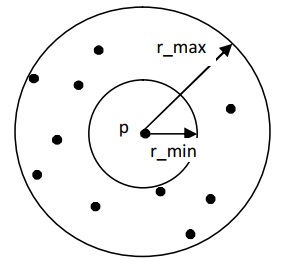
\includegraphics[width=0.25\textwidth]{Figures/radius.png} % Include the image .png
	\caption{Utilisation un pivot est de rayons de couvertures.}
\end{figure}

Dans la littérature, l’indexation de base de données par les méthodes d’accès métrique est conçue pour bénéficier d’une ou de plusieurs techniques discutées ci-dessus. On distinct entre deux approches : l’approche basée sur le partitionnement et l’approche basée sur les pivots (matrice des distances). Les méthodes basées sur les pivots construisent une matrice de distances entre les objets d’une région et les pivots afin de les utiliser pour filtrer les objets non pertinents lors de la recherche, tandis que, celle basées sur le partitionnement regroupent des objets similaires dans des régions, ce qui permet, lors de la recherche, d’éviter l’accès à des régions inutiles sans faire de calculs supplémentaires. Les taxonomie classiques souvent classifient les méthodes basées sur le partitionnent en deux catégories; le partitionnement par hyperplan et le partitionnement par boule [Chávez01]. Mais, plusieurs méthodes récentes ont dépassé cette classification soit par la proposition d’autres types de partitionnement ou par la combinaison de plusieurs types de partitionnement. \\

Plusieurs Méthodes d’accès métrique proposées en littérature sont basées sur l’idée de partitionnement des données. Elles peuvent se classifier sous quatre catégories; Les méthodes de partitionnement par boule, Les méthodes de partitionnement par hyperplan, Les méthodes de partitionnement par « Cut région » et les méthodes qui combinent plusieurs types de partitionnement [Hanif18].
\begin{figure}[H]
	\centering
	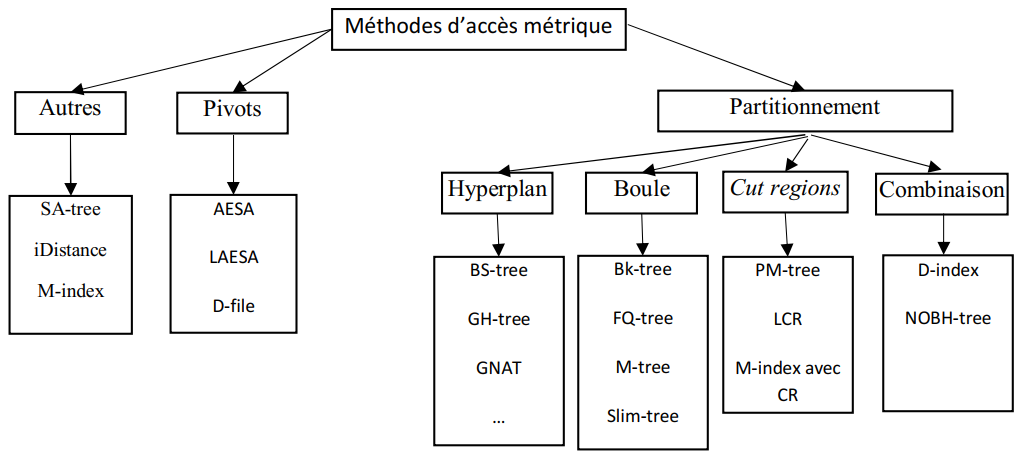
\includegraphics[width=0.55\textwidth]{Figures/class.png} % Include the image .png
	\caption{ Classification des méthodes d’accès métriques.}
\end{figure}
On s'intéresse principalement aux méthodes de partitionnement par boule.
Pour plus d'information sur les méthodes d'indexation, leurs avantages et inconvénients, le lecteur peut se référer à [Hanif18].
\section{La méthode partitionnement par boule M-tree}
Les méthodes de partitionnement en boule servent à partitionner l'espace des données sous formes des boules, elles utilisent des pivots et des rayons de couverture pour diviser les données. Le nombre des pivots utilisés, le choix du type de couverture des pivots font la différence entre les méthodes de partitionnement par boule, dans cette section nous présentons la méthodes de partitionnement par boules M-tree.

\subsection{La structuration de M-tree}
La méthode M-tree [CiPaZe97] est une structure efficace dans les environnements dynamiques caractérisés par un fréquent besoin de supprimer et d'ajouter des éléments. Le processus de construction de l'arbre M-tree consiste à partitionner l'espace métrique par des sphères région en se basant sur un pivot et un rayon de couverture. \\

M-Tree organise les objets en nœuds de taille fixe, qui correspondent aux régions de l'espace métrique. Les nœuds de l'arbre peuvent stocker jusqu'à \textbf{$ M $} entrées, c'est la capacité des nœuds. Les feuilles de l’arbre différent dans leur structure avec les nœuds internes:
\begin{itemize}
	\item Pour chaque objet indexé, une entrée au format 
	\begin{figure}[H]
		\centering
		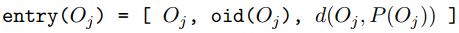
\includegraphics[width=0.6\textwidth]{entryleaf.png} % Include the image .png
	\end{figure} 
	est stockée dans un nœud feuille. Avec:
	\begin{itemize}
		\item \textbf{$ oid(O_j) $} est l'identifiant de l'objet qui réside dans un fichier de données séparé,
		\item \textbf{$ O_j $} sont les valeurs des caractéristiques de l'objet 
		\item et \textbf{$ d(O_j, P(O_j)) $} est la distance entre entre l’objet \textbf{$ O_j $} et l’objet  \textbf{$ P(O_j) $}, parent d'\textbf{$ O_j $}
	\end{itemize}

	\item Pour les nœuds internes, l'entrée stocké est au format
	\begin{figure}[H]
		\centering
		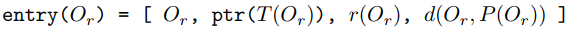
\includegraphics[width=0.7\textwidth]{entryInternal.png} % Include the image .png
	\end{figure} 
	Avec,
	\begin{itemize}
		\item \textbf{$ O_r $} est une valeur de caractéristique, également appelée un objet de routage,
		\item \textbf{$ r(O_r) $}$>0$ est un rayon de couverture, 
		\item \textbf{$ ptr(T( O_r)) $} est un pointeur à la racine du sous-arbre \textbf{$ T(O_r) $} - l'arbre couvrant d'\textbf{$ O_r $}, 
		\item et \textbf{$ d(O_r, P(O_r)) $} est la distance entre \textbf{$ O_j $} et \textbf{$ P(O_j) $}, l'objet parent d'\textbf{$ O_j $}\\
		
	\end{itemize}
\end{itemize}


La sémantique du rayon de recouvrement est exprimé par ce qui suit:
\begin{description}
	\item[Proprièté:] Le rayon de couverture d'un pivot (objet de routage), $ O_r $, satisfait l'inégalité $ d(O_j, O_r) \le r(O_r) $ pour chaque objet $ O_j $ stocké dans l'arbre de couverture de $ O_r $.
\end{description}

Un pivote définit donc une région dans l'espace métrique $ E $, centrée sur $ O_r $ et de rayon $ r(O_r) $, et $ O_r $ est le parent de chaque objet $ O_j $ stocké dans le nœud référencé par $ ptr(T(O_r)) $, c'est-à-dire $ O_r \equiv P(O_j)$ (voir figure 3.11 ).  Cela implique que le M-tree organise l'espace métrique en un ensemble de régions, qui peuvent se chevaucher, auxquelles le même principe est appliqué de manière récursive.

\begin{figure}[H]
	\centering
	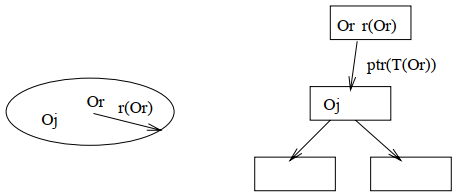
\includegraphics[width=0.55\textwidth]{Figures/mtree.png} % Include the image .png
	\caption{ Un pivot, $ O_r $, avec un rayon de couverture, $  r(O_r) $, qui référence le pivot suivant (sous arbre), $ T(O_r) $.}
\end{figure}

Les feuilles de l’arbre contiennent les identifiants des objets et leurs distances aux pivots associés, les nœuds internes mémorisent plusieurs paramètres comme le pointeur vers le pivot suivant, le rayon de couverture des régions de pivot concernés et un pointeur qui pointe vers le pivot fils. Chaque sous arbre contient les objets qui sont à une distance de pivot $ p $ inferieur au rayon de couverture.\\

\subsection{Comment M-tree grandit?}

Comme tout autre arbre dynamique équilibré (ou balancé), Le processus de construction de M-tree, qui se fait de bas en haut (un mode ascendant buttom-up), parcourt l'arbre à partir de la racine pour insérer le nouvel objet dans le sous arbre qui n'impose pas un changement de rayon de couverture. Si plusieurs sous arbre sont qualifiés, l'objet s'inséra dans le sous arbre de pivot le plus proche à l'objet inséré, sinon l'algorithme cherche le sous arbre qui peut avoir le minimum prolongement pour couvrir le nouvel objet.\\

M-tree est constitué d’un ensemble de nœuds de taille fixe $ M $, si l'insertion d'un objet produit un dépassement de capacité d'un nœud $ N $, le processus de construction fait appel à la fonction Split qui sert à créer un nouveau nœud $ N' $ de même niveau que le nœud saturé $ N  $ et d’appliquer un algorithme de redistribution de $ M+1 $ données entre l’ancien nœud et le nouveau nœud créer. Lorsque la racine se divise, une nouvelle racine est créée et l'arbre $ M $ grandit d'un niveau. La méthode Split est décrite de manière concise comme suit :\\

\begin{figure}[H]
	\centering
	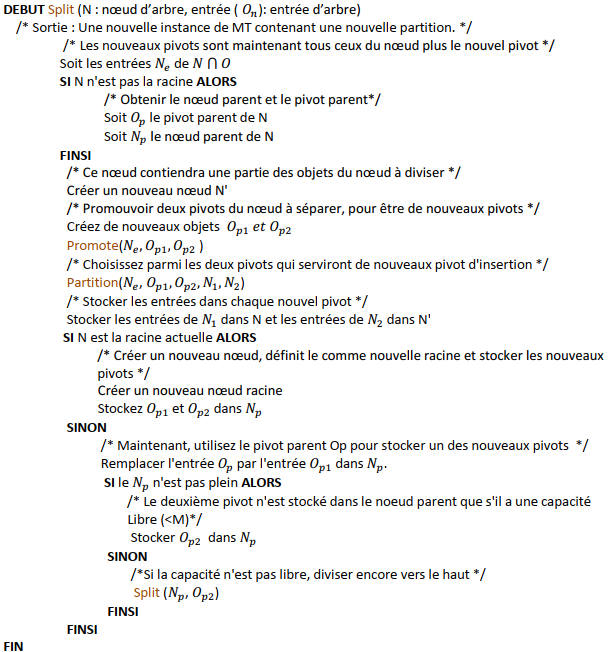
\includegraphics[width=0.95\textwidth]{Figures/split.png} % Include the image .png
\end{figure}

La méthode \textbf{Promote} choisit, en fonction de certains critères spécifiques, deux pivots, $ O_{p1} $ et $  O_{p2} $, à insérer dans le nœud parent, $ N_p $. La partition divise les $ (M + 1) $ entrées du nœud surchargé $ Ne $ en deux sous-ensembles disjoints, $ N_1 $ et $ N_2 $, qui sont ensuite stockés dans les nœuds $ N $ et $ N' $, respectivement. Une mise en œuvre spécifique de \textbf{Promote} et \textbf{Partition} définit ce que nous appelons une stratégie de fractionnement. Contrairement à d'autres modèles d'arbres métriques (statiques), chacun d'entre eux repose sur un critère spécifique d'organisation des objets, M-tree offre la possibilité de mettre en œuvre des stratégies de fractionnement alternatives, qui peuvent être ajustées en fonction des besoins de l'application \textbf{(voir section 3.5.5).}\\

Toute stratégie de fractionnement doit respecter la sémantique du rayon de couverture. Si le nœud du fractionnement, $ N $, est une feuille, cela est garanti par le paramétrage :

\begin{equation}
	r(O_{p1}) = \max \left\{d(O_j, O_{p1}) | O_j \in N_1 \right\}
\end{equation}

En général, le rayon de couverture d'un pivot pointant vers une feuille est égal à la distance maximale entre le pivot lui-même et les objets dans la feuille.\\

Lorsque la division implique un nœud interne, $ N $, chaque entrée $ O_j $ dans $ N_1 $ a un rayon de couverture non nul, $ r(O_j) $. En définissant:

\begin{equation}
r(O_{p1}) = \max \left\{d(O_j, O_{p1}) + r(O_j) | O_j \in N_1 \right\}
\end{equation}

Il est garanti, par la propriété d'inégalité triangulaire, qu'aucun objet dans $ T(O_{p1}) $ ne peut être distant de $  O_{p1} $ plus que $ r(O_{p1}) $. La figure 3.12 le montre dans le cas $ E = ( \mathbb{R^2}, L_2) $, c'est-à-dire le plan réel avec la distance euclidienne.
\begin{figure}[H]
	\centering
	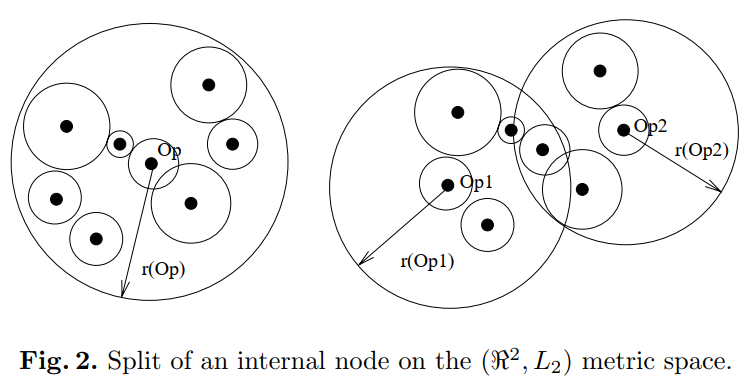
\includegraphics[width=.6 \textwidth]{Figures/splitexep.png} % Include the image .png
	\caption{Fractionnement d'un noeud interne dans l'espace  $ ( \mathbb{R^2}, L_2) $}
\end{figure} 

\subsection{Les requêtes de similarité}
Les algorithmes M-tree pour le traitement des requêtes de similarité visent à réduire le nombre de nœuds accessibles ainsi que le nombre de  de distances calculées. Cela est particulièrement important lorsque la recherche s'avère être orienté CPU, ce qui peut être le cas pour les fonctions de calcul de distance intensives. À cette fin, toutes les distances (pré-calculées) stockées dans les nœuds des M-trees, c'est-à-dire $ d(O_r, P(O_r)) $ et $ r(O_r) $, sont utilisées.

\subsubsection{Les requêtes intervalle (Range Queries)}
La requête $ range(Q, r(Q)) $ sélectionne tous les objets $ O_j $ de la base de données tels que $ d(O_j, Q) \le r(Q) $. L'algorithme \textbf{RangeSearch} part du nœud racine et parcourt récursivement tous les chemins qui ne peuvent pas être exclus pour aboutir à les objets qualifiants.
\begin{figure}[H]
	\centering
	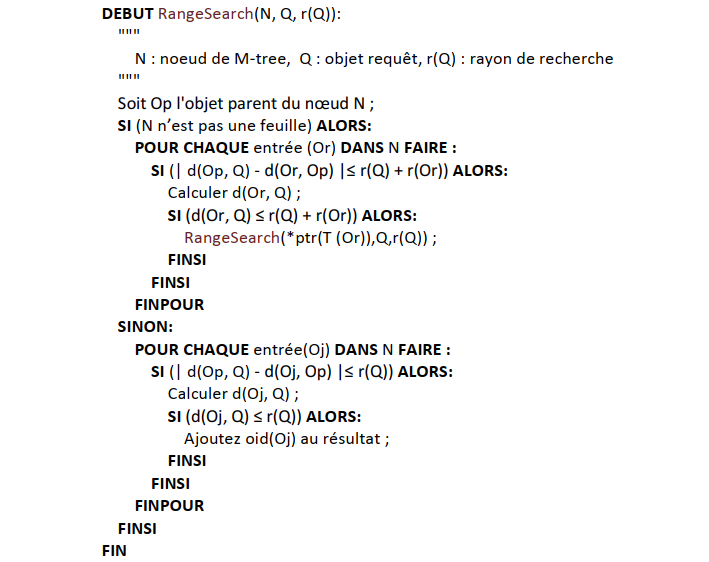
\includegraphics[width=.9 \textwidth]{Figures/rangesearxh.png} % Include the image .png
\end{figure} 

Comme, lors de l'accès au nœud $ N $, la distance entre $ Q $ et $ O_p $, l'objet parent de $ N $, a été déjà calculée, il est possible de se débarrasser d'un sous-arbre sans devoir calculer aucune nouvelle distance. La condition appliquée pour l'élagage (action de débarrasser) est la suivante.
\begin{description}
	\item[Lemme 1 :] Si $ d(O_r, Q) > r(Q) + r(O_r) $, alors, pour chaque objet $ O_j  $ dans $ T (O_r) $, c'est $ d(O_j, Q) > r(Q) $. Ainsi, $ T (O_r) $ peut être éliminé de la recherche en toute sécurité.
\end{description}
En fait, puisque $ d(O_j, Q) \ge d(O_r, Q) - d(O_j, O_r) $ (par l'inégalité triangulaire) et $ d(O_j, O_r) \le r(O_r) $ (par déf. du rayon de couverture), il s'agit de $ d(O_j, Q) \ge d(O_r, Q)-r(O_r) $.
Puisque, par hypothèse, il est $ d(O_r, Q) - r(O_r) > r(Q) $, le résultat suit.
Pour appliquer le Lemme 1, il faut calculer la distance $ d(O_r, Q) $. Cela peut être évité en tirant parti du résultat suivant.
\begin{description}
	\item[Lemme 2 :]  Si $ | d(O_p, Q) - d(O_r, Op) |> r(Q) + r(O_r) $, alors $ d(O_r, Q) > r(Q) + r(O_r) $.
\end{description}

C'est une conséquence directe de l'inégalité triangulaire, qui garantit que $ d(O_r, Q) \ge d(O_p, Q)-d(O_r, O_p) $ et$  d(O_r, Q) \ge d(O_r, O_p)-d(O_p, Q) $ sont tous les deux vrais (voir figure 3.13 en dessous). Le même principe d'optimisation est appliqué aux nœuds feuilles. Les résultats expérimentaux montrent que cette technique permet d'économiser jusqu'à 40\% de calculs de distances [CiPaZe97]. Le seul cas où les distances doivent nécessairement être calculées est celui du nœud racine, pour lequel l'$ O_p $ est indéfini.

\begin{figure}[H]
	\centering
	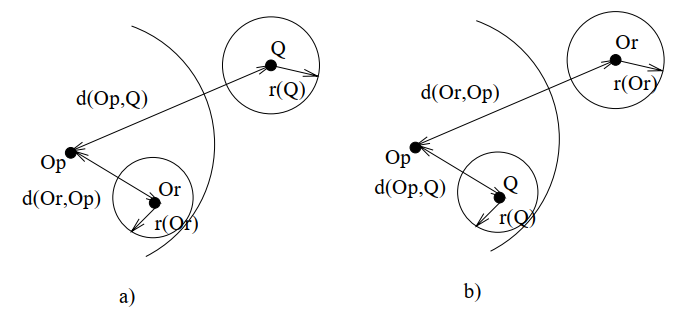
\includegraphics[width=.6 \textwidth]{Figures/lemme.png} % Include the image .png
	\caption{La figure montre comment le Lemme 2 est utilisé pour éviter de calculer les distances. \\Cas a) : $ d(O_r, Q) \ge d(O_p, Q) - d(O_r, O_p) > r(Q) + r(O_r) $ ; \\
		Cas b) : $ d(O_r, Q) \ge d(O_r, O_p) - d(O_p, Q) > r(Q) + r(O_r) $.}
\end{figure} 

\subsubsection{Les requêtes du k plus proche voisins (k-NN)}

L'algorithme de recherche k-NN (K Nearest Neighbors) récupère les k plus proches voisins d'un objet requête $ Q $ - on suppose qu'au moins $ k $ objets sont indexés par l'arbre M-tree. Nous utilisons une technique de branchement et de liaison(branch-and-bound), assez similaire à celle conçue pour les arbres R-tree [RKV95], qui utilise deux structures globales : une file d'attente prioritaire, \textbf{PR}, et un tableau de k éléments, \textbf{NN}, qui, à la fin de l'exécution, contiendra le résultat.\\

$ PR $ est une file d'attente de pointeurs vers des sous-arbres actifs, c'est-à-dire des sous-arbres où l'on peut trouver des objets qualifiants. Avec le pointeur vers (la racine du) sous-arbre $ T (O_r) $, une limite inférieure, $ d_{min}(T (O_r)) $, sur la distance de tout objet dans $ T (O_r) $ par rapport à $ Q $ est également conservée. La limite inférieure est

\begin{equation}
    d_{\min}(T(O_r)) = \max \left\{d(O_r, Q), 0\right\}
\end{equation}
puisqu'aucun objet dans $ T(O_r) $ ne peut avoir une distance de $  Q  $ inférieure à $ d(O_r, Q)-r(O_r) $.
Ces limites sont utilisées par la fonction \textit{ChooseNode} pour extraire de $ PR $ le noeud suivant à examiner. Comme le critère d'élagage de la recherche k-NN est dynamique - le rayon de recherche est la distance entre $ Q $ et son k-ième voisin le plus proche actuel - l'ordre dans lequel les nœuds sont visités peut affecter les performances. Le critère heuristique mis en œuvre par la fonction \textit{ChooseNode} consiste à sélectionner le nœud pour lequel la limite inférieure de $ d_{min} $ est minimale.(D'après les observations expérimentales, d'autres critères ne conduisent pas à une meilleure performance [CiPaZe97].).
\begin{figure}[H]
	\centering
	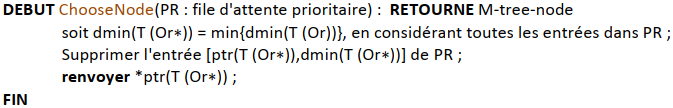
\includegraphics[width=.9 \textwidth]{Figures/choosenode.png} % Include the image .png
\end{figure} 


À la fin de l'exécution, la i-ième entrée du tableau $ NN $ aura la valeur $ NN[i] = [oid(O_j),d(O_j, Q)] $, $ O_j $ étant le i-ième voisin le plus proche de $ Q $. La valeur de la distance dans la i-ième entrée est désignée par $ d_i $, de sorte que $ d_k $ est la plus grande valeur de distance dans $ NN $. Il est clair que $ d_k $ joue le rôle d'un rayon de recherche dynamique, puisque tout sous-arbre pour lequel $ d_{min}(T(O_r)) > d_k $ peut être \textbf{élagué} en toute sécurité.\\

Les entrées du tableau $ NN $ sont initialement fixées à $ NN[i] = [null ,\infty] (i= 1,..., k) $, c'est-à-dire que les $ oid $ sont indéfinis et $ d_i = \infty $. Lorsque la recherche commence et que l'on accède aux nœuds (internes), l'idée est de calculer, pour chaque sous-arbre $ T(O_r) $, une limite supérieure, $ d_{max}(T(O_r)) $, sur la distance de tout objet dans $ T(O_r) $ par rapport à $ Q $. La limite supérieure est fixée à

\begin{equation}
d_{\max}(T(O_r)) =  d(O_r, Q)+r(O_r)
\end{equation}

Considérons le cas le plus simple $ k = 1 $, deux sous-arbres, $ T(O_{r1}) $ et $ T(O_{r2}) $, et supposons que $ dmax(T(O_{r1})) = 5 $ et $ dmin(T(O_{r2})) = 7 $. Puisque $ d_{max}(T(O_{r1})) $ garantit qu'un objet dont la distance de $  Q $ est au plus égale à 5 existe dans $ T(O_{r1}) $, $ T(O_{r2}) $ peut être élagué de la recherche. Les limites $ d_{max} $ sont insérées à des positions appropriées dans le tableau $ NN $, laissant juste le champ $ oid $ non défini. L'algorithme de recherche $ k-NN $ est donné ci-dessous.
\begin{figure}[H]
	\centering
	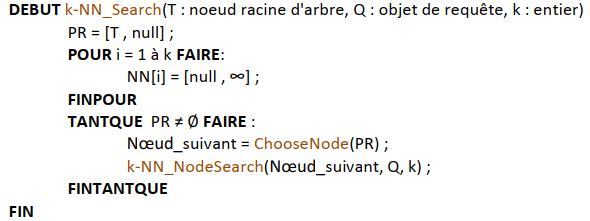
\includegraphics[width=.9 \textwidth]{Figures/knnsearch.png} % Include the image .png
\end{figure} 

La méthode \textit{k-NN-NodeSearch} implémente la majorité de la logique de recherche. Sur un nœud interne, elle détermine d'abord les sous-arbres actifs et les insère dans la file d'attente $ PR $. Ensuite, si nécessaire, elle appelle la fonction \textit{NN-Update} pour effectuer une insertion ordonnée dans le tableau $ NN $ et reçoit en retour un (possiblement nouvelle) valeur de $ d_k $. Cette valeur est ensuite utilisée pour retirer de $ PR $ tous les sous-arbres pour lesquels la limite inférieure de $ d_{min} $ dépasse $ d_{k} $. Des actions similaires sont effectuées dans les nœuds feuilles. Dans les deux cas l'optimisation visant à réduire le nombre de calculs de distance, qui utilise les distances pré-calculées de l'objet parent, est appliquée.

\begin{figure}[H]
	\centering
	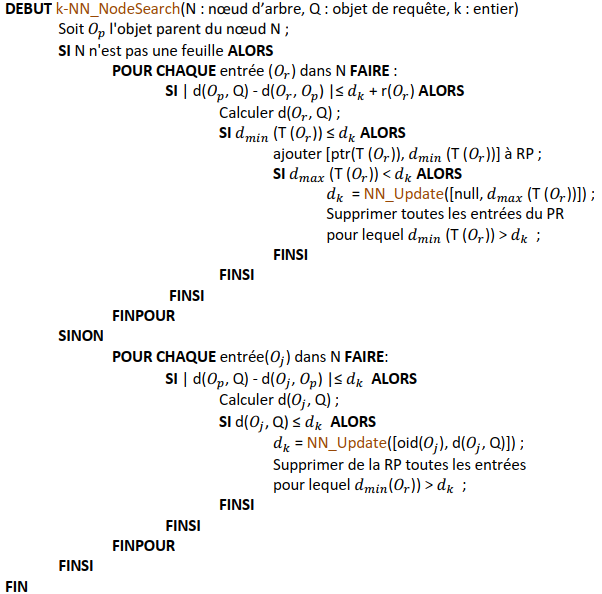
\includegraphics[width=.9 \textwidth]{Figures/knnnodesearch.png} % Include the image .png
\end{figure} 

\subsection{Insertion d'objets}
L'algorithme d'insertion descend récursivement l'arbre MT pour localiser le nœud feuille le plus approprié pour accueillir un nouvel objet, $ O_n $, déclenchant éventuellement une division si la feuille est pleine. Le raisonnement de base pour déterminer le nœud feuille "le plus approprié" est de descendre, à chaque niveau de l'arbre, le long d'un sous-arbre, $ T(O_r) $, pour lequel aucun élargissement du rayon de couverture n'est nécessaire, c'est-à-dire$  d(O_r, O_n) \le r(O_r) $. S'il existe plusieurs sous-arbres ayant cette propriété, on choisit celui pour lequel l'objet $ O_n $ est le plus proche de $ O_r $. Ce critère heuristique tente d'obtenir des sous-arbres bien regroupés, ce qui a un effet bénéfique sur les performances.\\

Si aucun pivot pour lequel $ d(O_r, O_n) \le r(O_r) $ existe - donc un rayon de couverture doit être élargi - notre choix est de minimiser l'augmentation du rayon de couverture, c'est-à-dire $ d(O_r, O_n)-r(O_r) $. Ceci est étroitement lié au critère heuristique qui suggère de minimiser le "volume" global couvert par les pivots dans le nœud actuel. L'algorithme Insert résume les arguments ci-dessus.
\begin{figure}[H]
	\centering
	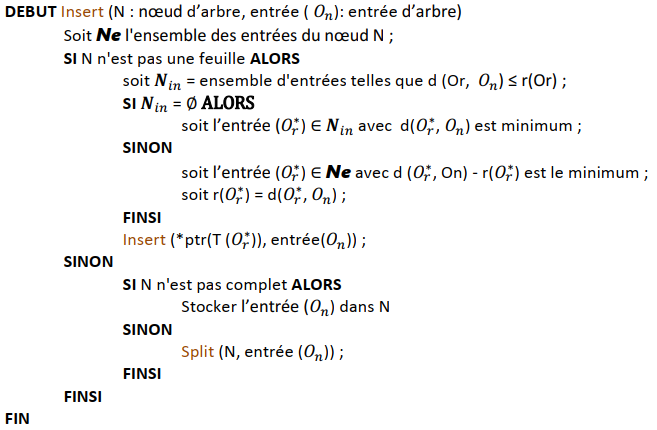
\includegraphics[width=.9 \textwidth]{Figures/insert.png} % Include the image .png
\end{figure} 


\subsection{Stratégies de fractionnement}
La stratégie de fractionnement "idéale" devrait sélectionner les deux objets à promouvoir, $ O_{p1} $ et $ O_{p2} $, et répartir les entrées de telle sorte que les deux régions ainsi obtenues aient un "volume" minimum et un "chevauchement" minimum. Ces deux critères visent à améliorer l'efficacité des algorithmes de recherche, car le fait d'avoir des régions de petite taille (faible volume) conduit à des arbres bien groupés et réduit la quantité d'espace inactif indexé - espace où aucun objet n'est présent - et le fait que le chevauchement entre les régions soit faible (voire nul) réduit le nombre de chemins à parcourir pour répondre à une requête.\\

Le critère du volume minimum conduit à concevoir des stratégies de fractionnement qui tentent de minimiser les valeurs des rayons de couverture, tandis que l'exigence de chevauchement minimum suggère que, pour des valeurs fixes des rayons de couverture, la distance entre les deux objets de référence choisis devrait être maximisée.

\subsubsection{Choix des pivots}
La méthode Promote détermine, à partir d'un ensemble d'entrées, $ Ne $ , deux objets à promouvoir et à stocker dans le nœud parent (voir section 3.5.2). Les algorithmes spécifiques que nous considérons peuvent d'abord être classés selon qu'ils "confirment" ou non l'objet parent dans son rôle.

\begin{description}
	\item[Définition]  Une stratégie de fractionnement confirmée choisit l'un des deux objets à promouvoir, par exemple l'$ O_{p1} $, pour être l'objet parent lui-même, $ O_p $, du nœud de fractionnement.
\end{description}

En d'autres termes, une stratégie de fractionnement confirmée ne fait que "extraire" une région, centrée sur le deuxième Pivot, l'$ O_{p2} $, de la région qui restera centrée sur l'$ O_p $. En général, cela simplifie l'exécution du fractionnement et réduit le nombre de calculs de distance.\\

Les alternatives que nous décrivons pour la mise en œuvre de Promote ne sont qu'un sous-ensemble sélectionné de l'ensemble que Ciaccia, Patella, Rabitti et Zezula ont évalué expérimentalement. Les autres stratégies sont décrit dans [CiPaZe97].

\begin{itemize}
	\item \textbf{m\_RAD :} L'algorithme du "minimum (sum of) RADius" est le plus complexe en termes de calcul de la distance. Il prend en compte toutes les paires d'objets possibles et, après avoir partitionné l'ensemble des entrées, promeut la paire d'objets pour laquelle la somme des rayons de couverture, $ r(O_{p1}) + r(O_{p2}) $, est minimale.
	\item \textbf{RANDOM :} Cette variante sélectionne simplement de manière aléatoire le ou les objets de référence.
	Bien que cette stratégie ne semble pas "intelligente", elle est rapide et ses performances peuvent servir de référence pour d'autres stratégies.
	\item \textbf{SAMPLING :} C'est la stratégie RANDOM, mais elle a été répétée sur un échantillon d'objets de taille $ s > 1 $. Pour chacune des paires d'objets $ s(s - 1)/2 $ de l'échantillon, les entrées sont réparties et des rayons de couverture potentiels sont établis. La paire pour laquelle la somme résultante des rayons de couverture, $ r(O_{p1})+r(O_{p2}) $, est minimale est alors sélectionnée.
	En cas de promotion confirmée, seules $ s $ différentes distributions sont essayées. Dans les expériences de [CiPaZe97], la taille de l'échantillon a été fixée à $ 1/10 $-ème de la capacité des nœuds.
	\item \textbf{M\_LB\_DIST :} L'acronyme signifie "Maximum Lower Bound on DISTance".
	Cette stratégie diffère des précédentes en ce sens qu'elle n'utilise que les distances stockées pré-calculées. Dans la version confirmée, où $ O_{p1} \equiv O_p $, l'algorithme détermine que l'$ O_{p2} $ est l'objet le plus éloigné de l'$ O_p $, c'est-à-dire:
	\begin{equation}
		 d(O_{p2}, O_p) = \max_j{d(O_j, O_p)}
	\end{equation}
	Lorsque $ O_{p1} = O_p $, les deux objets promus sont choisis de manière à ce que:
	\begin{equation}
	\makecell{d(O_{p1}, O_p) = \min_j{d(O_j, O_p)} \\
		 d(O_{p2}, O_p) = \max_j{d(O_j, O_p)}}
	\end{equation}
	La distance entre les deux pivots est alors garantie d'être au moins\\ $ d(O_{p2}, O_p)-d(O_{p1}, O_p) $, et aucun autre choix ne peut conduire à une limite supérieure.
\end{itemize}
Dans notre système nous avons choisi la dernière mèthode qui est M\_LB\_DIST.

\subsubsection{Répartition des entrées}
Étant donné un ensemble d'entrées $ Ne $ et les deux pivots $ O_{p1} $ et $ O_{p2} $, le problème est de savoir comment partitionner efficacement $ Ne $ en deux sous-ensembles, $  N_1 $ et $ N_2 $. À cette fin, nous envisager deux stratégies de base. La première est basée sur l'idée de la décomposition généralisée de l'hyperplan [Uhl91] et conduit à des fractionnements déséquilibrés, alors que la second obtient une répartition équilibrée. Ils peuvent être brièvement décrits comme suit.
\begin{itemize}
	\item \textbf{Hyperplan généralisé (Generalized Hyperplane) :} Assignez chaque objet $ O_j \in Ne $ au  pivot le plus proche, c'est-à-dire si $ d(O_j, O_{p1}) \le d(O_j, O_{p2}) $ alors assignez $ O_j $ à $ N_1 $, sinon assignez $ O_j $ à $ N_2 $.
	
	\item \textbf{Équilibré (Balanced) :} Calculer $ d(O_j, O_{p1}) $ et $ d(O_j, O_{p2}) $ pour tous les $ O_j \in Ne $ Répéter jusqu'à ce que $ Ne $ soit vide :\\
	 - Affecter à $ N_1 $ le plus proche voisin de l'$ O_{p1} $ dans $ Ne $ et le retirer de $ Ne $ ;\\
	 - Attribuer à $ N_2 $ le plus proche voisin de l'$ O_{p2} $ dans $ Ne $ et le retirer de $ Ne $.
\end{itemize}
En fonction de la distribution des données et de la manière dont les objets de routage sont choisis, une stratégie de fractionnement déséquilibrée peut conduire à un meilleur partitionnement des objets, en raison du degré de liberté supplémentaire que l'on obtient. En particulier, il faut remarquer que, si l'obtention d'un fractionnement équilibré avec des méthodes d'accès spatiale oblige à n'élargir les régions que selon les dimensions nécessaires, dans un espace métrique, l'augmentation conséquente du rayon de couverture se propagerait à toutes les "dimensions".\\

Un comportement intermédiaire peut être obtenu en combinant les deux algorithmes ci-dessus et en fixant un seuil minimum d'utilisation des nœuds. Si au moins $ m \le M/2 $ entrées par nœud sont nécessaires, la distribution équilibrée peut être appliquée aux 2 premiers $ m $ objets, après quoi l'hyperplan généralisé pourrait être utilisé. 

Pour en savoir plus sur l'évaluation des pérformances de la structures M-tree avec ses différentes types de requêtes et stratégies de fractionnement (partitionnement) le lecture peut consulter l'article [CiPaZe97].

\section{Conclusion}
Dans ce chapitres nous avons fait une études non exhaustive des méthodes d'indexations et leurs classifications. Pricipalement, nous avons présenté la structure d'accès métrique M-Tree et comment elle est construite, ainsi que ses algorithmes d'insertion et de recherche.

Généralement, la structure M-tree présente des avantages suivants: coût de recherche diminuer, dynamique, et résistance à l’augmentation de
la dimension. Mais, il peut présenter des chevauchement des nœuds [Hanif18].\\


Dans ce qui suit nous présenterons notre systèmes de recherche d'images par le contenu.

%
%
%
%La recherche par la requête intervalle R(q,r) d’un objet requête q et de rayon r dans M-tree exploite les distances pré-calculer pour éviter le parcours des nœuds inutiles. En effet, le processus de recherche commence par la racine, et pour chaque nœud visité: si la condition
%$ |d(q,p^p) — d(pp,^p)| — r^c > r $ est vérifiée alors on peut éviter le parcours du nœud sans faire des calculs supplémentaires, tel que $ d(q,p^p) $ est la distance entre la requête et l’objet père du nœud , $ d(p^p,p) $ est la distance entre l’objet p et l’objet père du nœud et $ r^c $ le rayon de couverture de nœud.
%
%La complexité de la construction de M-tree est d’ordre$  O(n.m^2.log_m n) $ telle que n est lenombre des distances stockées dans les feuilles et m représente la taille maximale des nœuds.


%P. Ciaccia, M. Patella, F. Rabitti, P. Zezula Indexing Metric Spaces with M-tree